% Options for packages loaded elsewhere
\PassOptionsToPackage{unicode}{hyperref}
\PassOptionsToPackage{hyphens}{url}
\PassOptionsToPackage{dvipsnames,svgnames,x11names}{xcolor}
%
\documentclass[
]{article}

\usepackage{amsmath,amssymb}
\usepackage{iftex}
\ifPDFTeX
  \usepackage[T1]{fontenc}
  \usepackage[utf8]{inputenc}
  \usepackage{textcomp} % provide euro and other symbols
\else % if luatex or xetex
  \usepackage{unicode-math}
  \defaultfontfeatures{Scale=MatchLowercase}
  \defaultfontfeatures[\rmfamily]{Ligatures=TeX,Scale=1}
\fi
\usepackage{lmodern}
\ifPDFTeX\else  
    % xetex/luatex font selection
\fi
% Use upquote if available, for straight quotes in verbatim environments
\IfFileExists{upquote.sty}{\usepackage{upquote}}{}
\IfFileExists{microtype.sty}{% use microtype if available
  \usepackage[]{microtype}
  \UseMicrotypeSet[protrusion]{basicmath} % disable protrusion for tt fonts
}{}
\makeatletter
\@ifundefined{KOMAClassName}{% if non-KOMA class
  \IfFileExists{parskip.sty}{%
    \usepackage{parskip}
  }{% else
    \setlength{\parindent}{0pt}
    \setlength{\parskip}{6pt plus 2pt minus 1pt}}
}{% if KOMA class
  \KOMAoptions{parskip=half}}
\makeatother
\usepackage{xcolor}
\setlength{\emergencystretch}{3em} % prevent overfull lines
\setcounter{secnumdepth}{5}
% Make \paragraph and \subparagraph free-standing
\makeatletter
\ifx\paragraph\undefined\else
  \let\oldparagraph\paragraph
  \renewcommand{\paragraph}{
    \@ifstar
      \xxxParagraphStar
      \xxxParagraphNoStar
  }
  \newcommand{\xxxParagraphStar}[1]{\oldparagraph*{#1}\mbox{}}
  \newcommand{\xxxParagraphNoStar}[1]{\oldparagraph{#1}\mbox{}}
\fi
\ifx\subparagraph\undefined\else
  \let\oldsubparagraph\subparagraph
  \renewcommand{\subparagraph}{
    \@ifstar
      \xxxSubParagraphStar
      \xxxSubParagraphNoStar
  }
  \newcommand{\xxxSubParagraphStar}[1]{\oldsubparagraph*{#1}\mbox{}}
  \newcommand{\xxxSubParagraphNoStar}[1]{\oldsubparagraph{#1}\mbox{}}
\fi
\makeatother


\providecommand{\tightlist}{%
  \setlength{\itemsep}{0pt}\setlength{\parskip}{0pt}}\usepackage{longtable,booktabs,array}
\usepackage{calc} % for calculating minipage widths
% Correct order of tables after \paragraph or \subparagraph
\usepackage{etoolbox}
\makeatletter
\patchcmd\longtable{\par}{\if@noskipsec\mbox{}\fi\par}{}{}
\makeatother
% Allow footnotes in longtable head/foot
\IfFileExists{footnotehyper.sty}{\usepackage{footnotehyper}}{\usepackage{footnote}}
\makesavenoteenv{longtable}
\usepackage{graphicx}
\makeatletter
\newsavebox\pandoc@box
\newcommand*\pandocbounded[1]{% scales image to fit in text height/width
  \sbox\pandoc@box{#1}%
  \Gscale@div\@tempa{\textheight}{\dimexpr\ht\pandoc@box+\dp\pandoc@box\relax}%
  \Gscale@div\@tempb{\linewidth}{\wd\pandoc@box}%
  \ifdim\@tempb\p@<\@tempa\p@\let\@tempa\@tempb\fi% select the smaller of both
  \ifdim\@tempa\p@<\p@\scalebox{\@tempa}{\usebox\pandoc@box}%
  \else\usebox{\pandoc@box}%
  \fi%
}
% Set default figure placement to htbp
\def\fps@figure{htbp}
\makeatother
% definitions for citeproc citations
\NewDocumentCommand\citeproctext{}{}
\NewDocumentCommand\citeproc{mm}{%
  \begingroup\def\citeproctext{#2}\cite{#1}\endgroup}
\makeatletter
 % allow citations to break across lines
 \let\@cite@ofmt\@firstofone
 % avoid brackets around text for \cite:
 \def\@biblabel#1{}
 \def\@cite#1#2{{#1\if@tempswa , #2\fi}}
\makeatother
\newlength{\cslhangindent}
\setlength{\cslhangindent}{1.5em}
\newlength{\csllabelwidth}
\setlength{\csllabelwidth}{3em}
\newenvironment{CSLReferences}[2] % #1 hanging-indent, #2 entry-spacing
 {\begin{list}{}{%
  \setlength{\itemindent}{0pt}
  \setlength{\leftmargin}{0pt}
  \setlength{\parsep}{0pt}
  % turn on hanging indent if param 1 is 1
  \ifodd #1
   \setlength{\leftmargin}{\cslhangindent}
   \setlength{\itemindent}{-1\cslhangindent}
  \fi
  % set entry spacing
  \setlength{\itemsep}{#2\baselineskip}}}
 {\end{list}}
\usepackage{calc}
\newcommand{\CSLBlock}[1]{\hfill\break\parbox[t]{\linewidth}{\strut\ignorespaces#1\strut}}
\newcommand{\CSLLeftMargin}[1]{\parbox[t]{\csllabelwidth}{\strut#1\strut}}
\newcommand{\CSLRightInline}[1]{\parbox[t]{\linewidth - \csllabelwidth}{\strut#1\strut}}
\newcommand{\CSLIndent}[1]{\hspace{\cslhangindent}#1}

\makeatletter
\@ifpackageloaded{caption}{}{\usepackage{caption}}
\AtBeginDocument{%
\ifdefined\contentsname
  \renewcommand*\contentsname{Table of contents}
\else
  \newcommand\contentsname{Table of contents}
\fi
\ifdefined\listfigurename
  \renewcommand*\listfigurename{List of Figures}
\else
  \newcommand\listfigurename{List of Figures}
\fi
\ifdefined\listtablename
  \renewcommand*\listtablename{List of Tables}
\else
  \newcommand\listtablename{List of Tables}
\fi
\ifdefined\figurename
  \renewcommand*\figurename{Figure}
\else
  \newcommand\figurename{Figure}
\fi
\ifdefined\tablename
  \renewcommand*\tablename{Table}
\else
  \newcommand\tablename{Table}
\fi
}
\@ifpackageloaded{float}{}{\usepackage{float}}
\floatstyle{ruled}
\@ifundefined{c@chapter}{\newfloat{codelisting}{h}{lop}}{\newfloat{codelisting}{h}{lop}[chapter]}
\floatname{codelisting}{Listing}
\newcommand*\listoflistings{\listof{codelisting}{List of Listings}}
\makeatother
\makeatletter
\makeatother
\makeatletter
\@ifpackageloaded{caption}{}{\usepackage{caption}}
\@ifpackageloaded{subcaption}{}{\usepackage{subcaption}}
\makeatother

\usepackage{bookmark}

\IfFileExists{xurl.sty}{\usepackage{xurl}}{} % add URL line breaks if available
\urlstyle{same} % disable monospaced font for URLs
\hypersetup{
  pdftitle={Methods for Reconstructing Paleo Food Webs},
  pdfauthor={Tanya Strydom; Andrew P. Beckerman},
  pdfkeywords={food web, network construction},
  colorlinks=true,
  linkcolor={blue},
  filecolor={Maroon},
  citecolor={Blue},
  urlcolor={Blue},
  pdfcreator={LaTeX via pandoc}}



\title{Methods for Reconstructing Paleo Food Webs}
\author{Tanya Strydom %
%
\textsuperscript{%
%
1%
}%
; Andrew P. Beckerman %
%
\textsuperscript{%
%
1%
}%
}
\date{2025-01-15}

\usepackage{setspace}
\usepackage[left]{lineno}
\usepackage[letterpaper]{geometry}

\usepackage[nolists,noheads,markers]{endfloat}
\geometry{margin=2.5cm}

\begin{document}

\thispagestyle{empty}
{\bfseries\sffamily\Large Methods for Reconstructing Paleo Food Webs}
\vfil
Tanya Strydom %
%
\textsuperscript{%
%
1%
}%
; Andrew P. Beckerman %
%
\textsuperscript{%
%
1%
}%

\vfil
{\small
\textbf{Abstract:} TODO.
\vfil
\textbf{Keywords:} %
food web, %
network construction%
}
\clearpage
\setcounter{page}{1}
\doublespacing
\linenumbers


\section{Why build paleo food webs?}\label{why-build-paleo-food-webs}

\begin{itemize}
\item
  Because its interesting?
\item
  Value in using hindcasting to aid in forecasting. \emph{e.g.,} the
  Toarcian ms (Dunhill et al., 2024) shows how we can use these paleo
  communities to understand trophic-level responses to extinctions.
\end{itemize}

\section{How do we do it?}\label{how-do-we-do-it}

\begin{itemize}
\item
  There is an evolving body of work that focuses on developing tools
  specifically for the task of predicting food webs.
\item
  There are a handful that have been developed specifically in the
  context of paleo settings \emph{e.g.,} TODO but we can also talk about
  those that might have been developed/tested in contemporary settings
  but still have applicability in paleo ones.
\item
  Different underlying theory though

  \begin{itemize}
  \tightlist
  \item
    Focus here on the idea of different `currencies' but also
    aggregations - energy vs compatibility.
  \end{itemize}
\item
  Insert brief overview of the different methods as they pertain to
  approach (so the T4T triangle)
\item
  Challenges we face (even in contemporary settings)?

  \begin{itemize}
  \tightlist
  \item
    keep high level - I think the argument here should fall more in the
    data trade offs\ldots{}
  \end{itemize}
\end{itemize}

\section{Understanding how networks are
different}\label{understanding-how-networks-are-different}

It is important to be aware that networks can be configured in different
ways depending on how the interactions are defined (Strydom, in prep).
Basically we have metawebs, which represent \emph{potential}
interactions, and realised networks, which represent the subset of
potential that are realised as a result of community and environmental
context.

\section{Challenges specific to paleo
communities/networks}\label{challenges-specific-to-paleo-communitiesnetworks}

Although there are a suite of tools and methods that have been developed
to predict species interactions and networks they will not all be
suitable for the prediction of paleo communities. Some of these include
the fact that the fossil record is incomplete/preservation is biased
{[}REF{]} which means that we have an incomplete picture of the entire
community. Fossils are 2D and only represent specific `parts' of an
individual (hard and bone-y bits), this means we don't have a complete
picture of the physical traits of species \emph{e.g.,} no body mass (but
yes size), behaviours, or ability to construct well resolved
phylogenetic trees the deeper we go back in time. Also owing to the
patchy nature of fossils one often has to aggregate over large spatial
scales, and also fossils are preserved in 2D so no \emph{real} idea of
spatial arrangements, compounded that fossils aren't necessarily
conserved/found `in situ' but can be moved (\emph{e.g.,} alluvial
deposits). Methodologically speaking some tools that `learn' from
contemporary communities (\emph{e.g.,} Strydom et al. (2023), Caron et
al. (2022)) will become `worse' the further one goes back in time since
species then look very different from now but can still be useful for
`recent' communities (\emph{e.g.,} Fricke et al. (2022)). Something
about the intersectionality of the data we don't have for paleo
communities and the data we need for some of the different modelling
approaches.

\section{Dataset Overview}\label{dataset-overview}

\begin{itemize}
\item
  Species
\item
  Time/space
\item
  And probably some other paleo things that will be relevant\ldots{}
\end{itemize}

\begin{figure}[H]

{\centering \pandocbounded{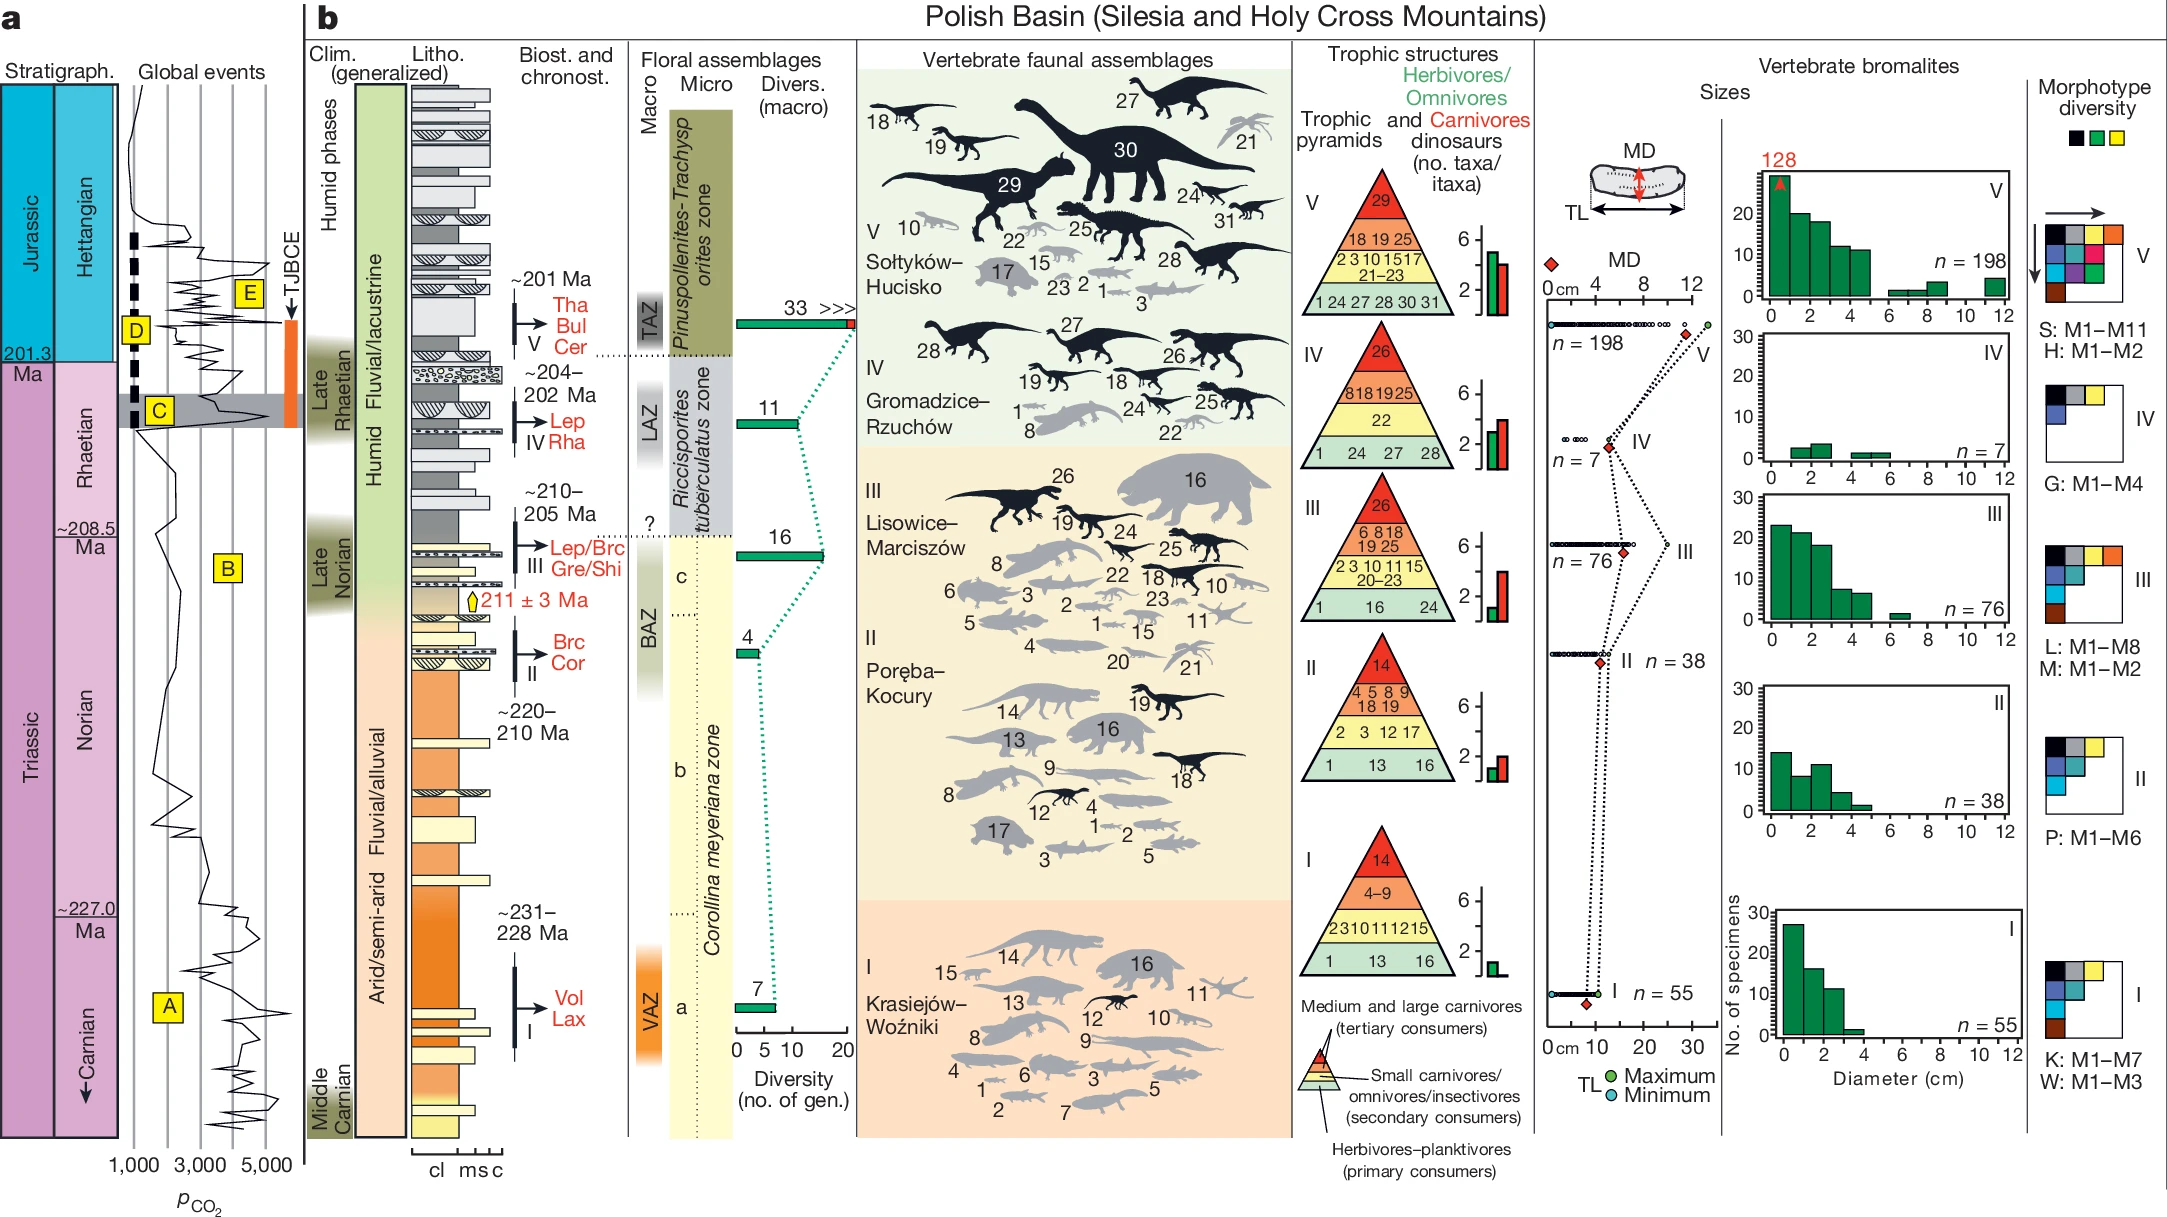
\includegraphics[keepaspectratio]{figures/data_mock.png}}

}

\caption{It would be very sexy if we could get a figure that looks
something like this together\ldots{}}

\end{figure}%

\section{Methods}\label{methods}

\subsection{Models}\label{models}

\begin{longtable}[]{@{}
  >{\raggedright\arraybackslash}p{(\linewidth - 4\tabcolsep) * \real{0.2639}}
  >{\raggedright\arraybackslash}p{(\linewidth - 4\tabcolsep) * \real{0.2917}}
  >{\raggedright\arraybackslash}p{(\linewidth - 4\tabcolsep) * \real{0.4444}}@{}}
\caption{A summary of the different families of tools that can be used
to generate paleo food webs.}\label{tbl-models}\tabularnewline
\toprule\noalign{}
\begin{minipage}[b]{\linewidth}\raggedright
Model
\end{minipage} & \begin{minipage}[b]{\linewidth}\raggedright
Predicts
\end{minipage} & \begin{minipage}[b]{\linewidth}\raggedright
Notes
\end{minipage} \\
\midrule\noalign{}
\endfirsthead
\toprule\noalign{}
\begin{minipage}[b]{\linewidth}\raggedright
Model
\end{minipage} & \begin{minipage}[b]{\linewidth}\raggedright
Predicts
\end{minipage} & \begin{minipage}[b]{\linewidth}\raggedright
Notes
\end{minipage} \\
\midrule\noalign{}
\endhead
\bottomrule\noalign{}
\endlastfoot
Allometric diet breadth model & Realised network & \\
Body size ratio model & Metaweb (?) & \\
Niche model & Structural network & Is not species specific - cannot
apply species metadata \\
Paleo food web inference model & Realised network (if downsampling) & \\
\end{longtable}

\subsubsection{Paleo food web inference
model}\label{paleo-food-web-inference-model}

The Paleo food web inference model (PFIM; Shaw et al. (2024)) uses a
series of rules for a set of trait categories (such as habitat and body
size) to determine if an interaction can feasibly occur between a
species pair. If all conditions are met for the different rule classes
then an interaction is deemed to be feasible. The original work put
forward in Shaw et al. (2024) also includes a `downsampling' step
developed by Roopnarine (2006) that uses a power law, defined by the
link distribution, to `prune' down some of the links. It is worth
mentioning that this approach is similar to that developed by Roopnarine
(2017) with the exception that Shaw does not specifically bin species
into guilds, and so we choose to use the method developed by Shaw since
both methods should produce extremely similar networks as they are built
on the same underlying philosophy.

\paragraph{Defining organism ecologies, feeding interactions and trophic
guilds}\label{defining-organism-ecologies-feeding-interactions-and-trophic-guilds}

\begin{quote}
This is currently verbatim from the Dunhill ms\ldots{}
\end{quote}

Modes of life were defined for each fossil species based on the
ecological traits defined in the Bambach ecospace model (Bambach et al.,
2007). Ecological traits were assigned based on interpretations from the
published literature which are largely based on functional morphology
and information from extant relatives. Information on the body size of
each species was also recorded by summarising mean specimen sizes from
the section into a categorical classification. The following ecological
characteristics were recorded for each fossil species; motility (fast,
slow, facultative, non-motile), tiering (pelagic, erect, surficial,
semi-infaunal, shallow infaunal, deep infaunal), feeding (predator,
suspension feeder, deposit feeder, mining, grazer), and size: gigantic
(\textgreater500 mm), very large (\textgreater300--500 mm), large
(\textgreater100--300 mm), medium (\textgreater50--100 mm), small
(\textgreater10--50 mm), tiny (≤10 mm). Size categories are defined by
the longest axis of the fossil, estimates of tracemaker size from trace
fossils based on literature accounts, or by extrapolating the total
length for belemnites from the preserved guard using established
approaches.

\subsubsection{Allometric diet breadth
model}\label{allometric-diet-breadth-model}

The Allometric diet breadth model (ADBM; Petchey et al. (2008)) is
rooted in feeding theory and allocates the links between species based
on energetics, which predicts the diet of a consumer based on energy
intake. This means that the model is focused on predicting not only the
number of links in a network but also the arrangement of these links
based on the diet breadth of a species, where the diet (\(K\)) is
defined as follows:

\begin{equation}\phantomsection\label{eq-adbm}{
K = \frac{\sum_{i=1}^{k}\lambda_{ij}E_{i}}{1+\sum_{i=1}^{k}\lambda_{ij}H_{ij}}
}\end{equation}

where \(\lambda_{ij}\) is the handling time, which is the product of the
attack rate \(A_{i}\) and resource density \(N_{i}\), \(E_{i}\) is the
energy content of the resource and \(H_{ij}\) is the ratio handling
time, with the relationship being dependent on the ratio of predator and
prey bodymass as follows:

\[
H_{ij} = \frac{h}{b - \frac{M_{i}}{M_{j}}} if \frac{M_{i}}{M_{j}} < b
\]

or

\[
H_{ij} = \infty \geq b
\]

Refer to Petchey et al. (2008) for more details as to how these
different terms are parametrised.

\subsubsection{Body size ratio model}\label{body-size-ratio-model}

The body size ratio model (Rohr et al., 2010) determines feeding
interactions using the ratio between consumer (\(M_{i}\)) and resource
(\(M_{j}\)) body sizes - which supposedly stems from niche theory (still
trying to reconcile that). The probability of a link existing between a
consumer and resource (in its most basic form) is defined as follows:

\[
P_{ij} = \frac{p}{1+p}
\]

where

\begin{equation}\phantomsection\label{eq-bodymass}{
p = exp[\alpha + \beta log(\frac{M_{i}}{M_{j}}) + \gamma log^{2}(\frac{M_{i}}{M_{j}})]
}\end{equation}

The original latent-trait model developed by Rohr et al. (2010) also
included an additional latent trait term \(v_{i} \delta f_{j}\) however
for simplicity we will use Equation~\ref{eq-bodymass} as per Yeakel et
al. (2014) Based on Rohr et al. (2010) it is possible to estimate the
parameters \(\alpha\), \(\delta\), and \(\gamma\) using a GLM but we
will use the parameters from Yeakel et al. (2014), which was `trained'
on the Serengeti food web data and are as follows: \(\alpha\) = 1.41,
\(\delta\) = 3.75, and \(\gamma\) = 1.87.

\subsubsection{L matrix}\label{l-matrix}

For now we can link to thATNr package (Gauzens et al., 2023) until I can
find a more suitable manuscript that breaks down this construction
method. Schneider et al. (2016) Interactions are determined by
allometric rules (ratio of consumer (\(M_{i}\)) and resource (\(M_{j}\))
body sizes) and a Ricker function as defined by \(R_{opt}\) and
\(\gamma\) and returns The probability of a link (\(P_{ij}\)) existing
between a consumer and resource, and is defined as follows:

\[
P_{ij} = (L \times \exp(1 - L))^{\gamma}
\]

where

\[
L = \frac{M_{i}}{M_{j} \times R_{opt}}
\]

It is also possible to apply a threshold value to \(P_{ij}\), whereby
any probabilities below that threshold are set to zero.

\subsubsection{Niche model}\label{niche-model}

The niche model (Williams \& Martinez, 2000) introduces the idea that
species interactions are based on the `feeding niche' of a species.
Broadly, all species are randomly assigned a `feeding niche' range and
all species that fall in this range can be consumed by that species
(thereby allowing for cannibalism). The niche of each species is
randomly assigned and the range of each species' niche is (in part)
constrained by the specified connectance of the network. The niche model
has also been modified, although it appears that adding to the
`complexity' of the niche model does not improve on its ability to
generate a more ecologically `correct' network (Williams \& Martinez,
2008).

\subsection{Assessing model
performance}\label{assessing-model-performance}

In terms of wanting to asses and compare across the different models it
is beneficial to approach this task by thinking about the different
aspects of the network as well as interactions that are being predicted
by the different models. It is perhaps beneficial to think of these
across different `scales' of organisation within the network, namely
macro (the entire network), meso (smaller interacting units within the
network), and micro (species-level attributes). Although there are a
myriad of possible ways to `measure' and analyse ecological networks
(Delmas et al., 2018) we do still lack a clear set of guidelines for
assessing how well models recover network structure (Allesina et al.,
2008) and it is beneficial to use a small subset of metrics that can
clearly be tied to broader aspects of network function or capturing a
ecological process.

\subsubsection{Macro network properties}\label{macro-network-properties}

\textbf{Connectance} (Martinez, 1992) has been shown to be the feature
of networks that underpin a series of other properties and function
(Strydom, Catchen, et al., 2021) and so it is perhaps the most important
structural attribute for a model to be able to retrieve correctly.
Additionally we consider the \textbf{complexity} of networks by
calculating their SVD entropy (this gives us an estimate of the physical
as opposed to behavioural complexity of networks; Strydom, Dalla Riva,
et al. (2021)), we could also look at the rank/rank deficiency of
networks which (theoretically) represents the number fo unique
interaction strategies in the network (Strydom, Dalla Riva, et al.,
2021), which may be specifically interesting in terms of looking at pre
and post extinction but also as a way to unpack `functional redundancy'
that some models may introduce.

\subsubsection{Meso network properties}\label{meso-network-properties}

Motifs represent smaller subset of interactions between three species,
and are argued to capture dynamics that are likely to be ecologically
relevant (Milo et al., 2002; Stouffer et al., 2007). Here we
specifically look at the number of \textbf{linear chains},
\textbf{omnivory}, \textbf{apparent competition}, and \textbf{direct
competition} motifs. In the broader context the ability of a model in
being able to capture these smaller motifs will inform as to its
suitability of use understanding the more dynamic component of network
ecology.

\subsubsection{Micro network properties}\label{micro-network-properties}

The number of interactions established (\textbf{generality}) or received
(\textbf{vulnerability}) by each species (Schoener, 1989), are (broadly)
indicative of consumer-resource relationships and diet breadth of
species {[}ref{]}. Although this is usually determined at the species
level the standard deviation of the generality and vulnerability of
species is often used when benchmarking predicted networks (Petchey et
al., 2008; \emph{e.g.,} Williams \& Martinez, 2008).

The \textbf{specificity} of species in a network is measured as a
function of the proportion of resources they effectively use (Poisot et
al., 2012)

\begin{quote}
\textbf{Shape:} to determine if the `shape' of the network is correct we
are looking at the ratio of `top':`basal' species (where `top' species
are those that have a vulnerability of 0 and `basal' species have a
generality of 0) as well as the distance to base from one of the top
species (this will represent the shortest path but a large discrepancy
between the real and predicted network would be indicative that the
model is not predicting a similar `shape'). This will allow is to see if
the models construct tall `pencil' vs flat `pancake' networks (Beckerman
2024, pers comms). A small (\textless{} 1) number will thus be
indicative of a `bottom-heavy' network and the opposite for larger
numbers
\end{quote}

\subsubsection{Interactions}\label{interactions}

\textbf{Interaction turnover} (Poisot et al., 2012) tells us which
interactions are `conserved' (shared) across the networks from the same
period but constructed using different models.

\section{Results}\label{results}

\subsection{Comparing predicted
networks}\label{comparing-predicted-networks}

\begin{figure}

\centering{

\pandocbounded{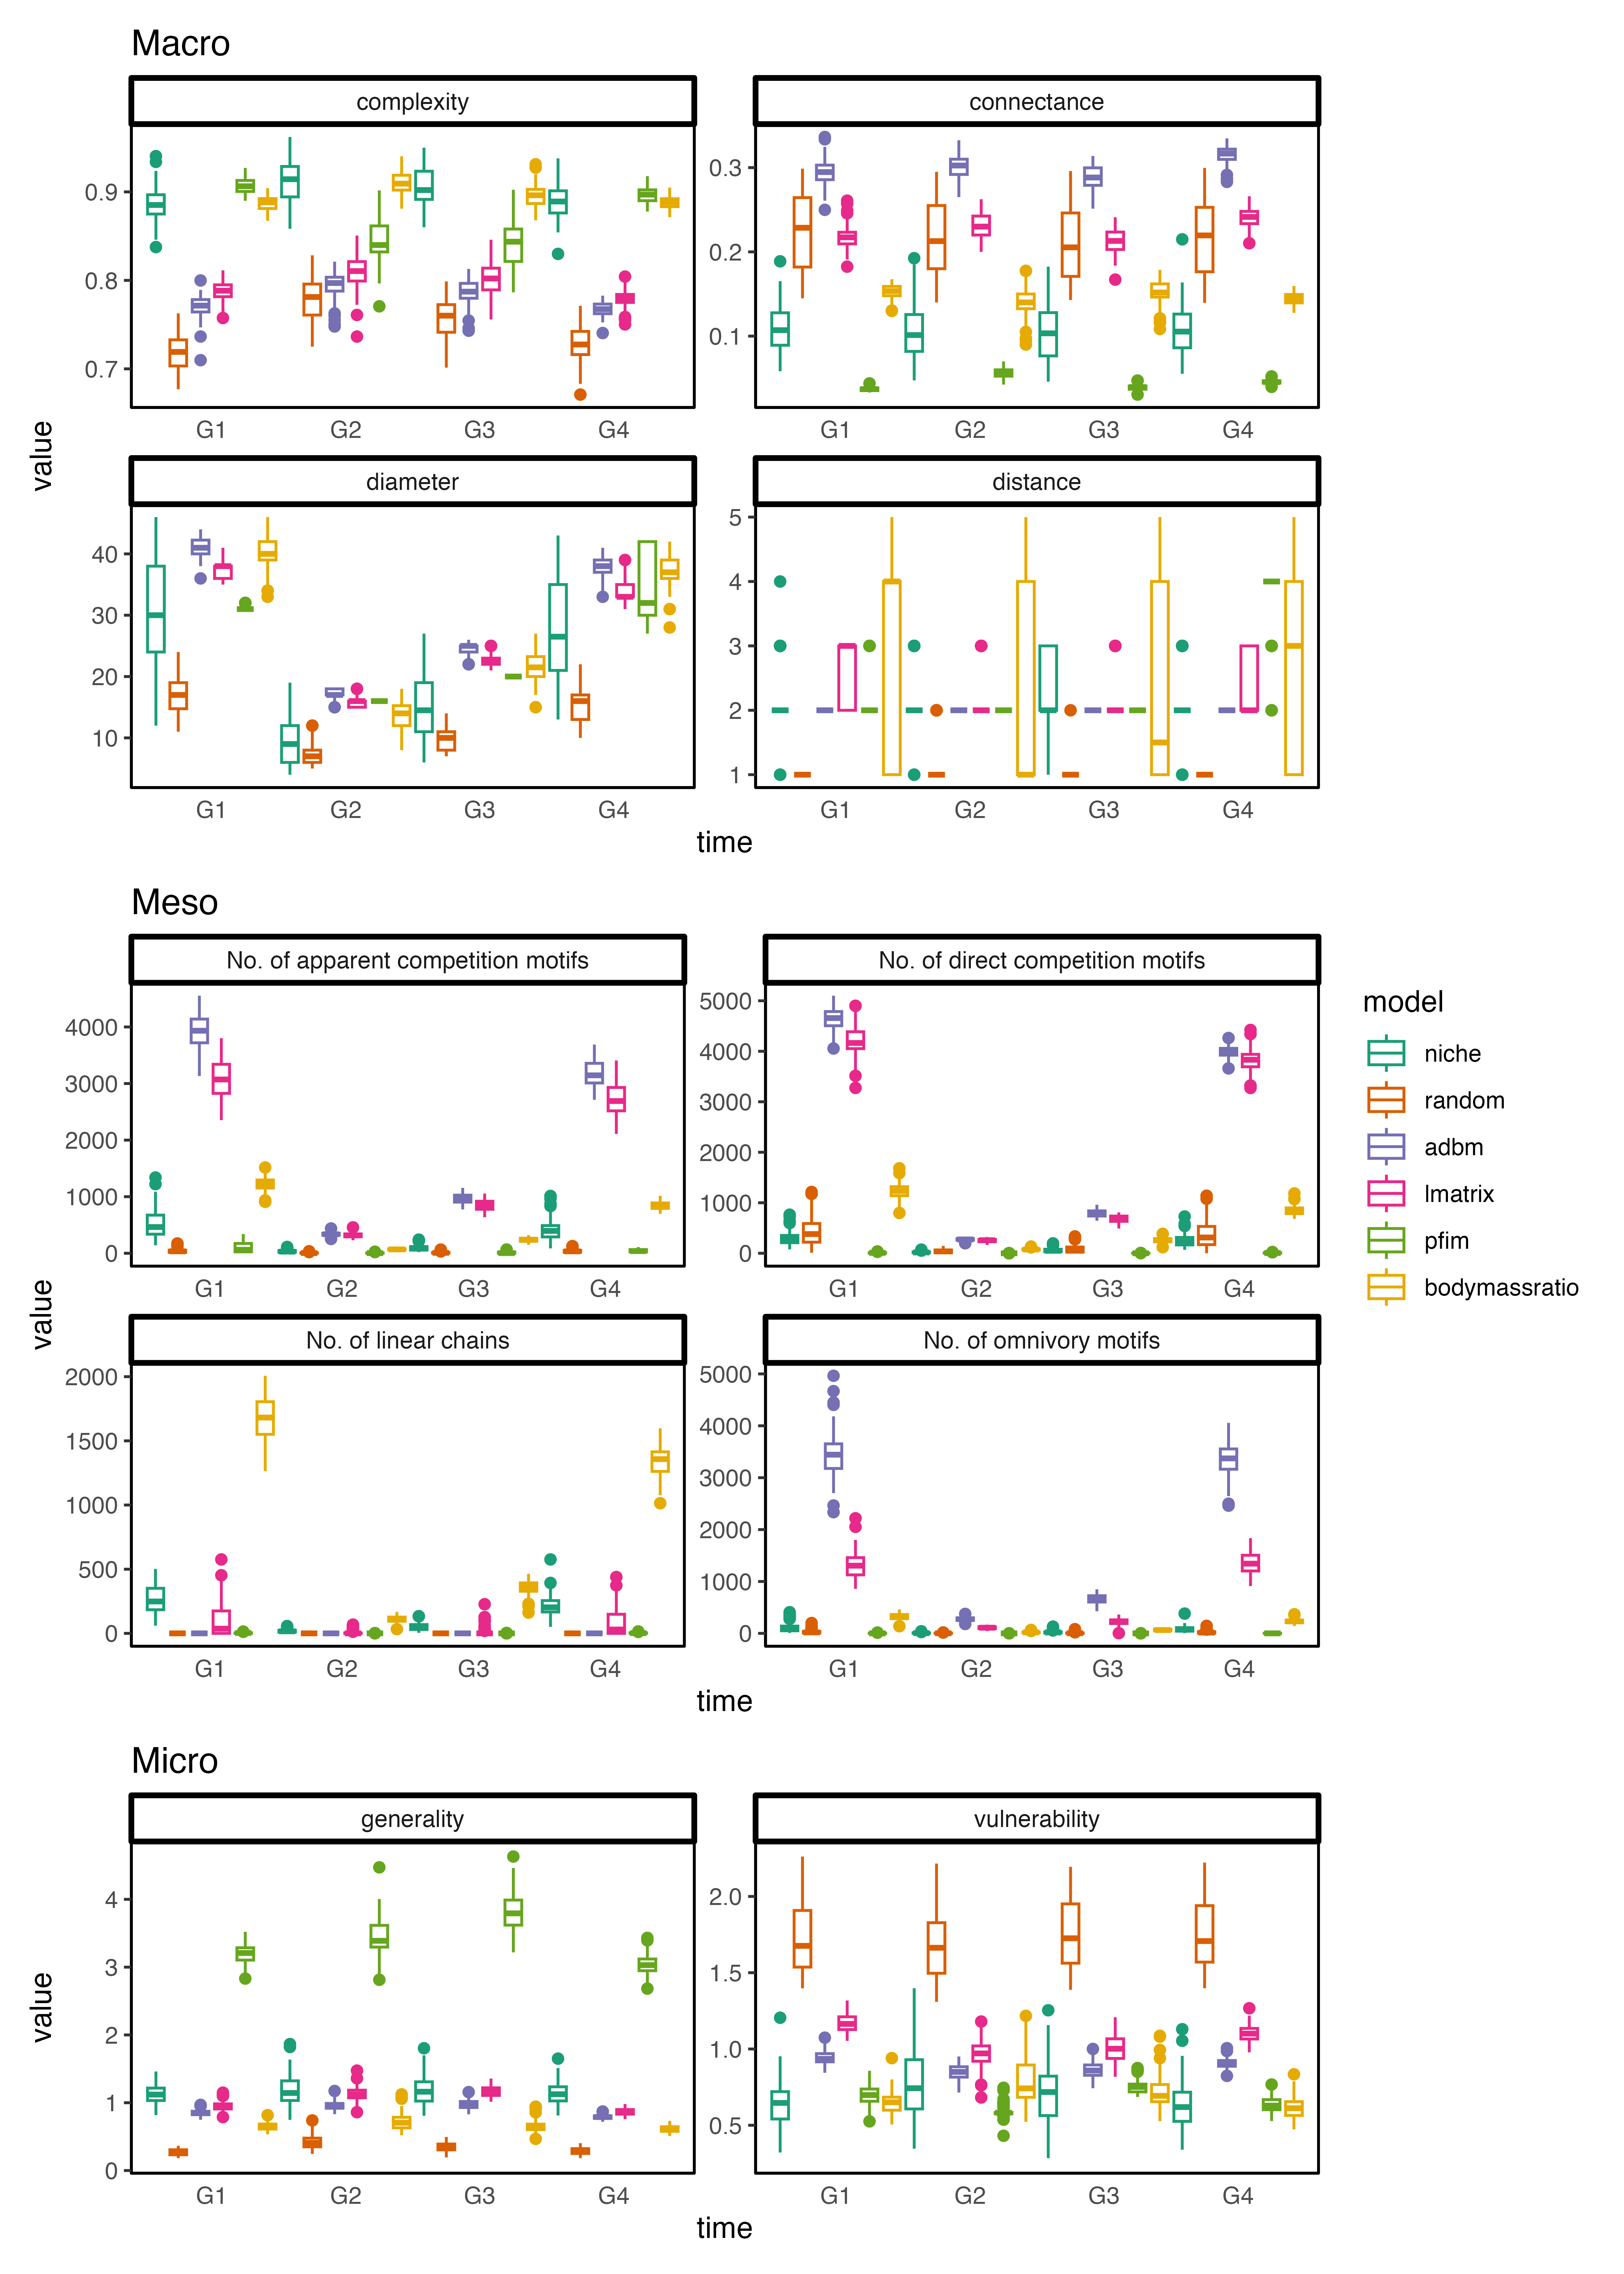
\includegraphics[keepaspectratio]{figures/summary.png}}

}

\caption{\label{fig-summary}stuff\ldots{} For display purposes the
counts for the different motifs are log transformed}

\end{figure}%

\subsection{Comparing inference}\label{comparing-inference}

\subsection{Extinctions}\label{extinctions}

\begin{figure}

\centering{

\pandocbounded{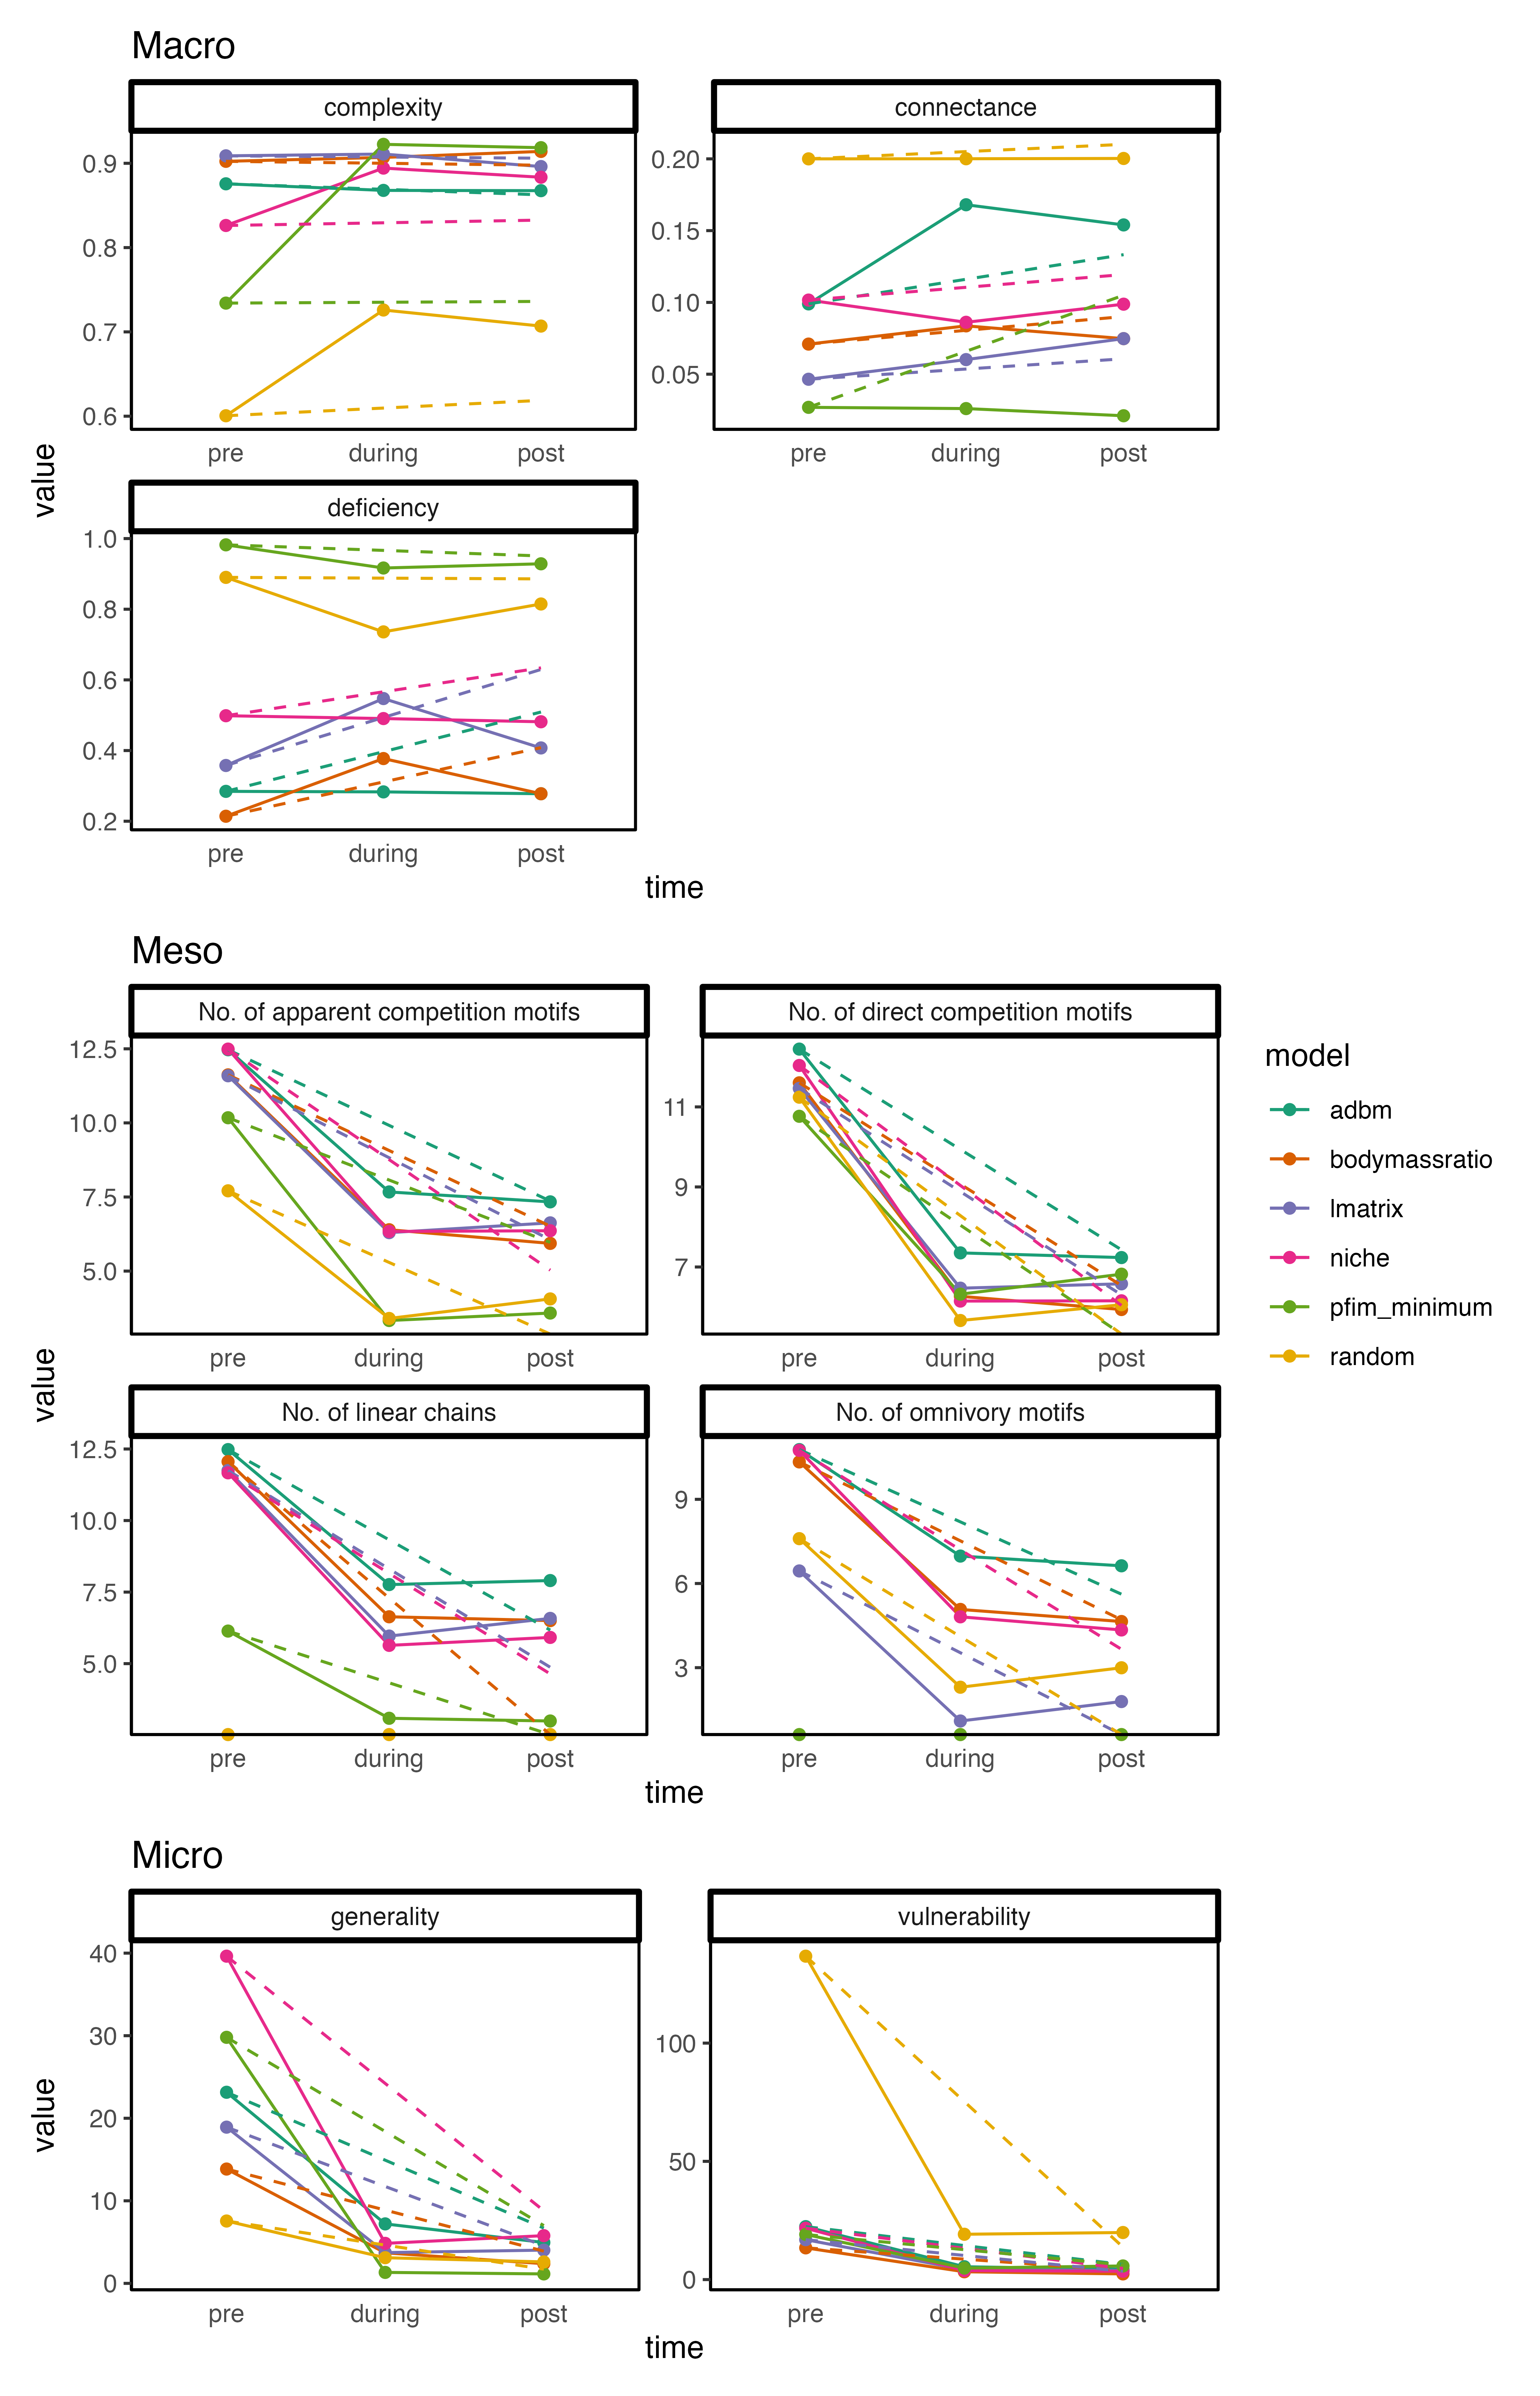
\includegraphics[keepaspectratio]{figures/extinction.png}}

}

\caption{\label{fig-extinction}Dashed line indicates the (mean)
extinction simulation results (post value, start values are those
estimated by the relevant model). For display purposes the counts for
the different motifs are log transformed}

\end{figure}%

\begin{figure}[H]

{\centering \pandocbounded{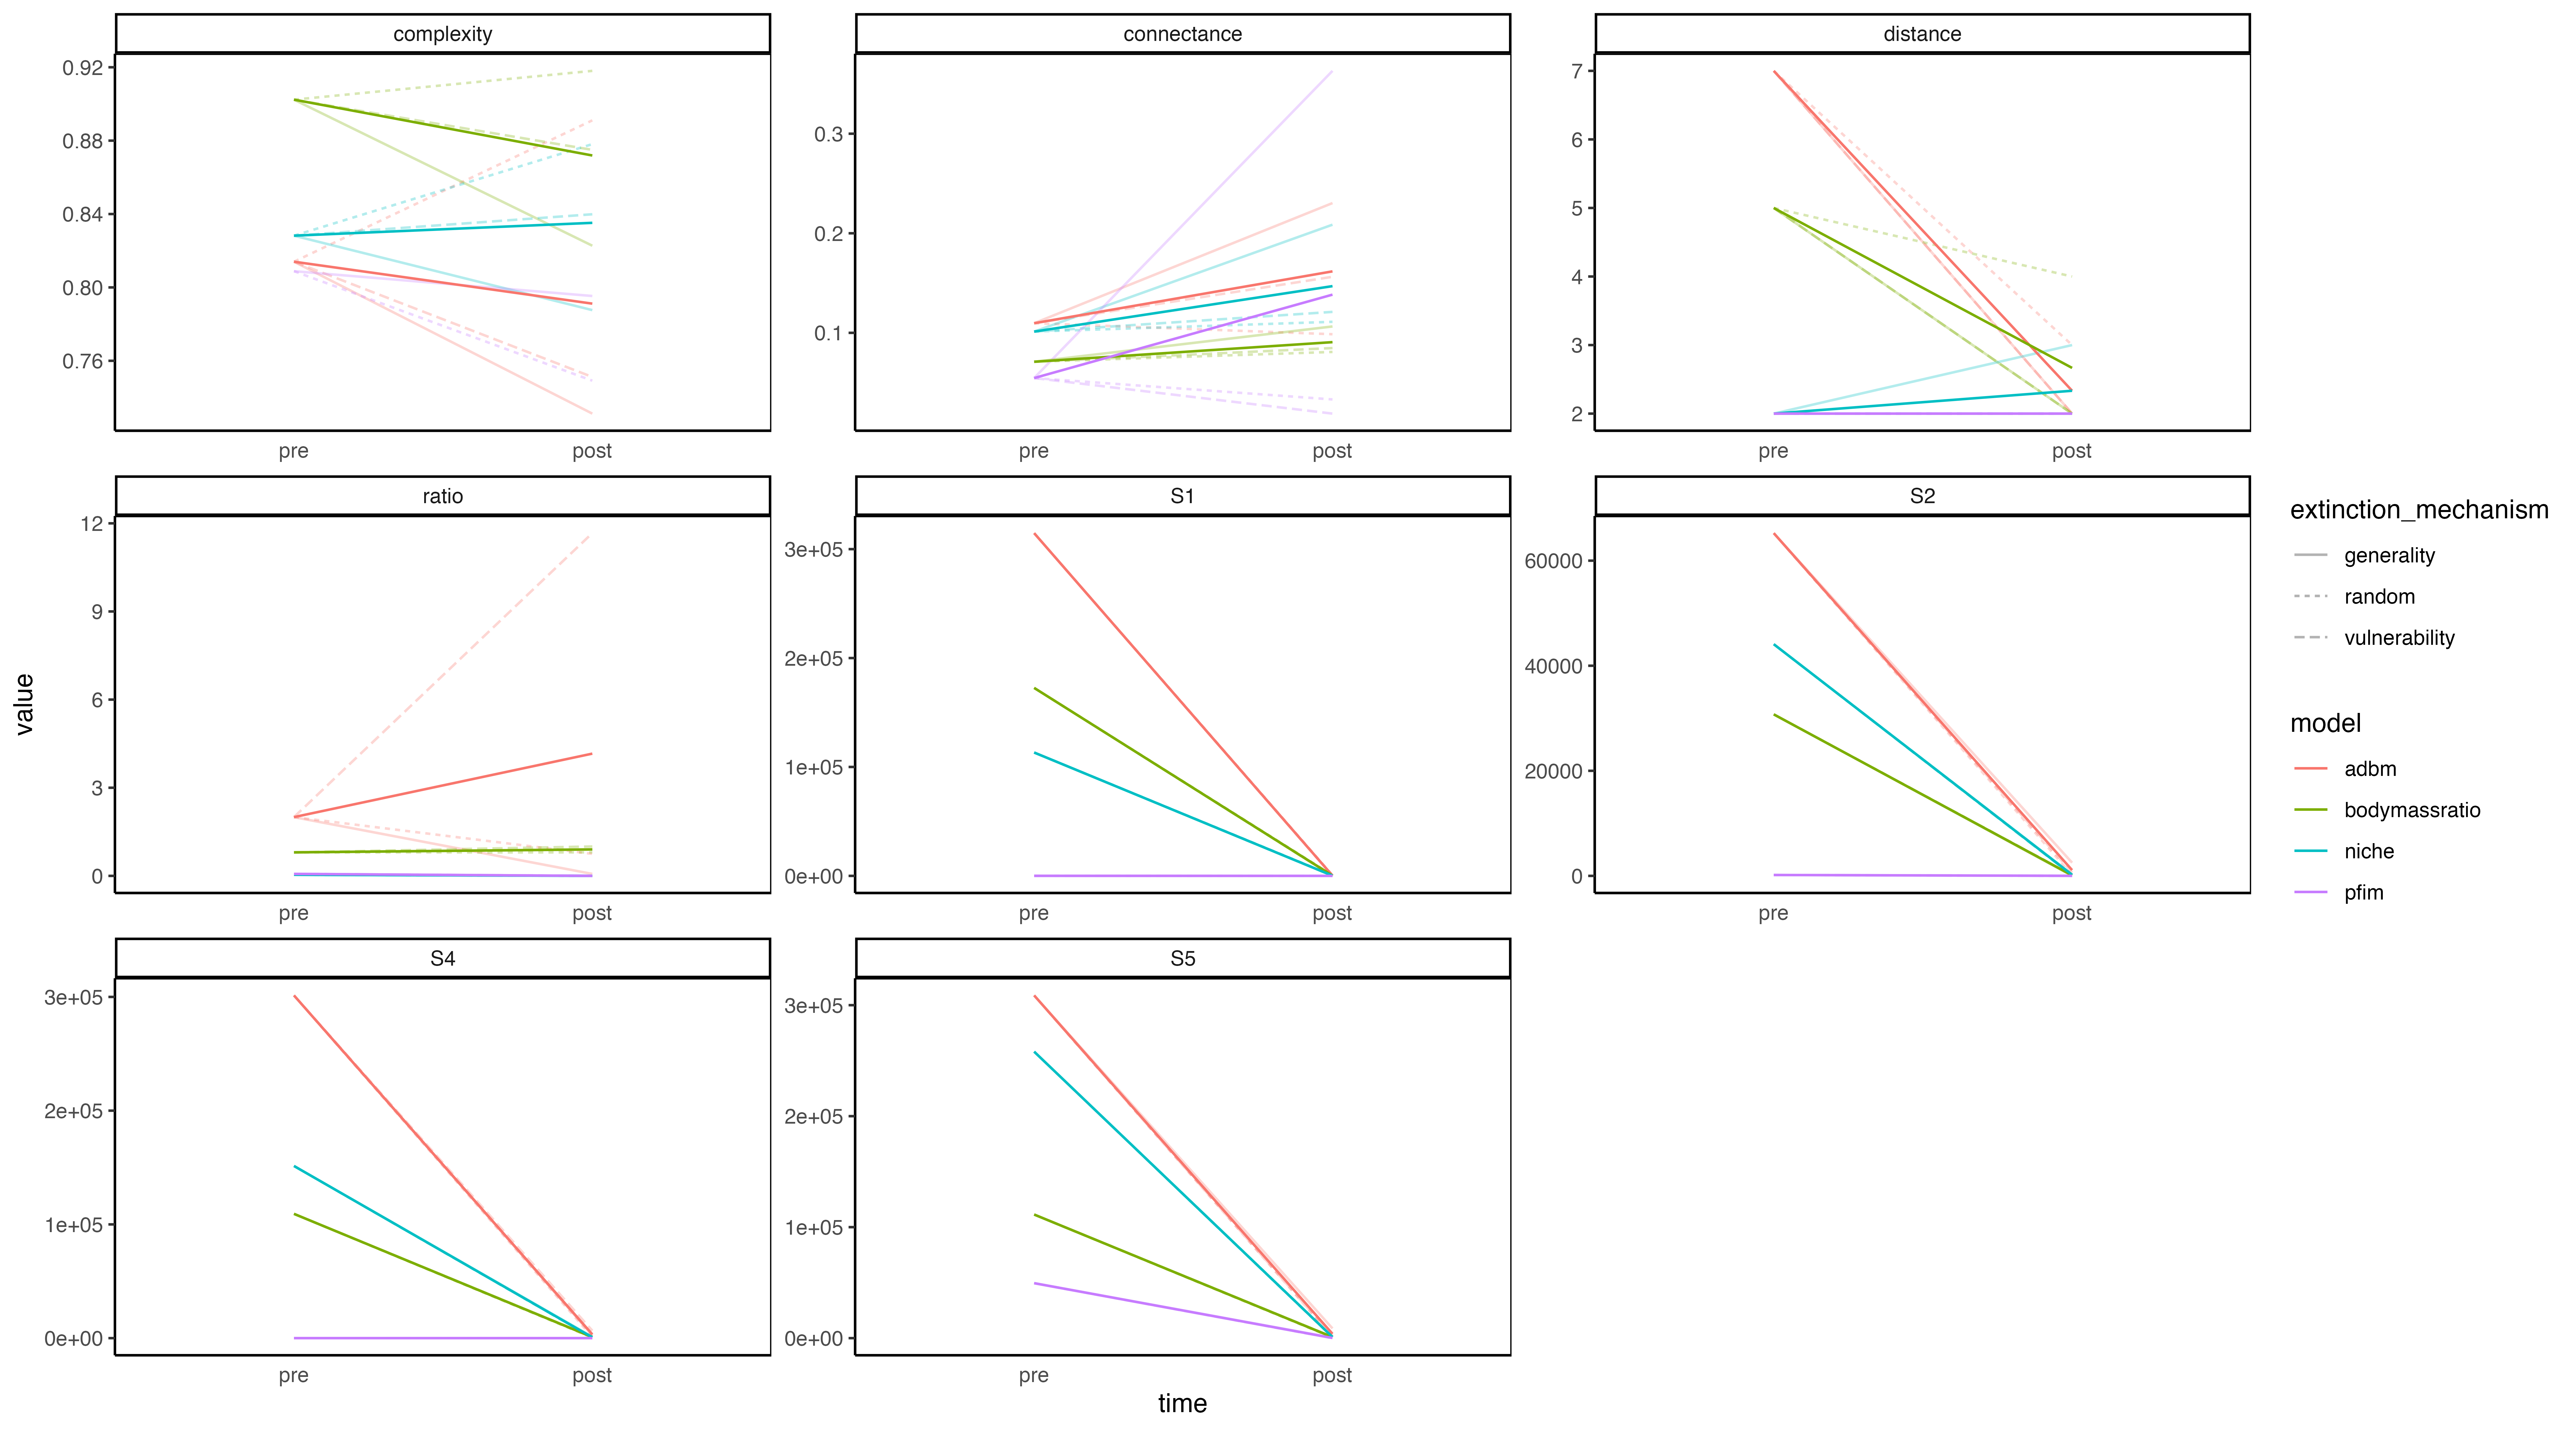
\includegraphics[keepaspectratio]{figures/extinction_all_results.png}}

}

\caption{Dark line indicates `real' extinction simulation results the
lighter lines show each model individually, which is also denoted by the
linetype. For display purposes the counts for the different motifs are
log transformed}

\end{figure}%

\section*{References}\label{references}
\addcontentsline{toc}{section}{References}

\phantomsection\label{refs}
\begin{CSLReferences}{1}{0}
\bibitem[\citeproctext]{ref-allesina2008}
Allesina, S., Alonso, D., \& Pascual, M. (2008). A general model for
food web structure. \emph{Science}, \emph{320}(5876), 658--661.
\url{https://doi.org/10.1126/science.1156269}

\bibitem[\citeproctext]{ref-bambach2007}
Bambach, R. K., Bush, A. M., \& Erwin, D. H. (2007). Autecology and the
Filling of Ecospace: Key Metazoan Radiations. \emph{Palaeontology},
\emph{50}(1), 1--22.
\url{https://doi.org/10.1111/j.1475-4983.2006.00611.x}

\bibitem[\citeproctext]{ref-caron2022}
Caron, D., Maiorano, L., Thuiller, W., \& Pollock, L. J. (2022).
Addressing the Eltonian shortfall with trait-based interaction models.
\emph{Ecology Letters}, \emph{25}(4), 889--899.
\url{https://doi.org/10.1111/ele.13966}

\bibitem[\citeproctext]{ref-delmas2018}
Delmas, E., Besson, M., Brice, M.-H., Burkle, L. A., Dalla Riva, G. V.,
Fortin, M.-J., Gravel, D., Guimarães, P. R., Hembry, D. H., Newman, E.
A., Olesen, J. M., Pires, M. M., Yeakel, J. D., \& Poisot, T. (2018).
Analysing ecological networks of species interactions. \emph{Biological
Reviews}, 112540. \url{https://doi.org/10.1111/brv.12433}

\bibitem[\citeproctext]{ref-dunhill2024}
Dunhill, A. M., Zarzyczny, K., Shaw, J. O., Atkinson, J. W., Little, C.
T. S., \& Beckerman, A. P. (2024). Extinction cascades, community
collapse, and recovery across a Mesozoic hyperthermal event.
\emph{Nature Communications}, \emph{15}(1), 8599.
\url{https://doi.org/10.1038/s41467-024-53000-2}

\bibitem[\citeproctext]{ref-fricke2022}
Fricke, E. C., Hsieh, C., Middleton, O., Gorczynski, D., Cappello, C.
D., Sanisidro, O., Rowan, J., Svenning, J.-C., \& Beaudrot, L. (2022).
Collapse of terrestrial mammal food webs since the Late Pleistocene.
\emph{Science}, \emph{377}(6609), 1008--1011.
\url{https://doi.org/10.1126/science.abn4012}

\bibitem[\citeproctext]{ref-gauzens2023}
Gauzens, B., Brose, U., Delmas, E., \& Berti, E. (2023). ATNr:
Allometric Trophic Network models in R. \emph{Methods in Ecology and
Evolution}, \emph{14}(11), 2766--2773.
\url{https://doi.org/10.1111/2041-210X.14212}

\bibitem[\citeproctext]{ref-martinez1992}
Martinez, N. D. (1992). Constant connectance in community food webs.
\emph{The American Naturalist}, \emph{139}(6), 1208--1218.
\url{http://www.jstor.org/stable/2462337}

\bibitem[\citeproctext]{ref-milo2002}
Milo, R., Shen-Orr, S., Itzkovitz, S., Kashtan, N., Chklovskii, D., \&
Alon, U. (2002). Network motifs: Simple building blocks of complex
networks. \emph{Science}, \emph{298}(5594), 824--827.
\url{https://doi.org/10.1126/science.298.5594.824}

\bibitem[\citeproctext]{ref-petchey2008}
Petchey, O. L., Beckerman, A. P., Riede, J. O., \& Warren, P. H. (2008).
Size, foraging, and food web structure. \emph{Proceedings of the
National Academy of Sciences}, \emph{105}(11), 4191--4196.
\url{https://doi.org/10.1073/pnas.0710672105}

\bibitem[\citeproctext]{ref-poisot2012}
Poisot, T., Canard, E., Mouquet, N., \& Hochberg, M. E. (2012). A
comparative study of ecological specialization estimators. \emph{Methods
in Ecology and Evolution}, \emph{3}(3), 537--544.
\url{https://doi.org/10.1111/j.2041-210x.2011.00174.x}

\bibitem[\citeproctext]{ref-rohr2010}
Rohr, R., Scherer, H., Kehrli, P., Mazza, C., \& Bersier, L.-F. (2010).
Modeling food webs: Exploring unexplained structure using latent traits.
\emph{The American Naturalist}, \emph{176}(2), 170--177.
\url{https://doi.org/10.1086/653667}

\bibitem[\citeproctext]{ref-roopnarine2006}
Roopnarine, P. D. (2006). Extinction cascades and catastrophe in ancient
food webs. \emph{Paleobiology}, \emph{32}(1), 1--19.
\url{https://www.jstor.org/stable/4096814}

\bibitem[\citeproctext]{ref-roopnarine2017}
Roopnarine, P. D. (2017). \emph{Ecological Modelling of Paleocommunity
Food Webs} (pp. 201--226). University of Chicago Press.

\bibitem[\citeproctext]{ref-schneider2016}
Schneider, F. D., Brose, U., Rall, B. C., \& Guill, C. (2016). Animal
diversity and ecosystem functioning in dynamic food webs. \emph{Nature
Communications}, \emph{7}(1), 12718.
\url{https://doi.org/10.1038/ncomms12718}

\bibitem[\citeproctext]{ref-schoener1989}
Schoener, T. W. (1989). Food Webs From the Small to the Large: The
Robert H. MacArthur Award Lecture. \emph{Ecology}, \emph{70}(6),
1559--1589. \url{https://doi.org/10.2307/1938088}

\bibitem[\citeproctext]{ref-shaw2024}
Shaw, J. O., Dunhill, A. M., Beckerman, A. P., Dunne, J. A., \& Hull, P.
M. (2024). \emph{A framework for reconstructing ancient food webs using
functional trait data} (p. 2024.01.30.578036). bioRxiv.
\url{https://doi.org/10.1101/2024.01.30.578036}

\bibitem[\citeproctext]{ref-stouffer2007}
Stouffer, D. B., Camacho, J., Jiang, W., \& Nunes Amaral, L. A. (2007).
Evidence for the existence of a robust pattern of prey selection in food
webs. \emph{Proceedings of the Royal Society B: Biological Sciences},
\emph{274}(1621), 1931--1940.
\url{https://doi.org/10.1098/rspb.2007.0571}

\bibitem[\citeproctext]{ref-strydom2023}
Strydom, T., Bouskila, S., Banville, F., Barros, C., Caron, D., Farrell,
M. J., Fortin, M.-J., Mercier, B., Pollock, L. J., Runghen, R., Dalla
Riva, G. V., \& Poisot, T. (2023). Graph embedding and transfer learning
can help predict potential species interaction networks despite data
limitations. \emph{Methods in Ecology and Evolution}, \emph{14}(12),
2917--2930. \url{https://doi.org/10.1111/2041-210X.14228}

\bibitem[\citeproctext]{ref-strydom2021b}
Strydom, T., Catchen, M. D., Banville, F., Caron, D., Dansereau, G.,
Desjardins-Proulx, P., Forero-Muñoz, N. R., Higino, G., Mercier, B.,
Gonzalez, A., Gravel, D., Pollock, L., \& Poisot, T. (2021). A roadmap
towards predicting species interaction networks (across space and time).
\emph{Philosophical Transactions of the Royal Society B: Biological
Sciences}, \emph{376}(1837), 20210063.
\url{https://doi.org/10.1098/rstb.2021.0063}

\bibitem[\citeproctext]{ref-strydom2021}
Strydom, T., Dalla Riva, G. V., \& Poisot, T. (2021). SVD entropy
reveals the high complexity of ecological networks. \emph{Frontiers in
Ecology and Evolution}, \emph{9}.
\url{https://doi.org/10.3389/fevo.2021.623141}

\bibitem[\citeproctext]{ref-williams2000}
Williams, R. J., \& Martinez, N. D. (2000). Simple rules yield complex
food webs. \emph{Nature}, \emph{404}(6774), 180--183.
\url{https://doi.org/10.1038/35004572}

\bibitem[\citeproctext]{ref-williams2008}
Williams, R. J., \& Martinez, N. D. (2008). Success and its limits among
structural models of complex food webs. \emph{The Journal of Animal
Ecology}, \emph{77}(3), 512--519.
\url{https://doi.org/10.1111/j.1365-2656.2008.01362.x}

\bibitem[\citeproctext]{ref-yeakel2014}
Yeakel, J. D., Pires, M. M., Rudolf, L., Dominy, N. J., Koch, P. L.,
Guimarães, P. R., \& Gross, T. (2014). Collapse of an ecological network
in ancient egypt. \emph{PNAS}, \emph{111}(40), 14472--14477.
\url{https://doi.org/10.1073/pnas.1408471111}

\end{CSLReferences}





\end{document}
